%%%%%%%%%%%%%%%%%%%%%%%%%%%%%%%%%%%%%%%%%%%%%%%%%%%%%%%%%%%%%%%%%%%%%%%%%%%%%%%%%%%%%%%
%%%%%%%%%%%%%%%%%%%%%%%%%%%%%%%%%%%%%%%%%%%%%%%%%%%%%%%%%%%%%%%%%%%%%%%%%%%%%%%%%%%%%%%
% 
% This top part of the document is called the 'preamble'.  Modify it with caution!
%
% The real document starts below where it says 'The main document starts here'.

\documentclass[12pt]{article}

\usepackage{amssymb,amsmath,amsthm}
\usepackage[top=1in, bottom=1in, left=1.25in, right=1.25in]{geometry}
\usepackage{fancyhdr}
\usepackage{enumerate}
\usepackage{listings}
\usepackage{graphicx}
\usepackage{float}
\usepackage{multirow}

\usepackage{mwe}
\usepackage{caption}
\usepackage{subcaption}
% Comment the following line to use TeX's default font of Computer Modern.
\usepackage{times,txfonts}



\makeatletter
\renewcommand*\env@matrix[1][*\c@MaxMatrixCols c]{%
  \hskip -\arraycolsep
  \let\@ifnextchar\new@ifnextchar
  \array{#1}}
\makeatother

\newtheoremstyle{homework}% name of the style to be used
  {18pt}% measure of space to leave above the theorem. E.g.: 3pt
  {12pt}% measure of space to leave below the theorem. E.g.: 3pt
  {}% name of font to use in the body of the theorem
  {}% measure of space to indent
  {\bfseries}% name of head font
  {:}% punctuation between head and body
  {2ex}% space after theorem head; " " = normal interword space
  {}% Manually specify head
\theoremstyle{homework} 

% Set up an Exercise environment and a Solution label.
\newtheorem*{exercisecore}{Exercise \@currentlabel}
\newenvironment{exercise}[1]
{\def\@currentlabel{#1}\exercisecore}
{\endexercisecore}

\newcommand{\localhead}[1]{\par\smallskip\noindent\textbf{#1}\nobreak\\}%
\newcommand\solution{\localhead{Solution:}}

%%%%%%%%%%%%%%%%%%%%%%%%%%%%%%%%%%%%%%%%%%%%%%%%%%%%%%%%%%%%%%%%%%%%%%%%
%
% Stuff for getting the name/document date/title across the header
\makeatletter
\RequirePackage{fancyhdr}
\pagestyle{fancy}
\fancyfoot[C]{\ifnum \value{page} > 1\relax\thepage\fi}
\fancyhead[L]{\ifx\@doclabel\@empty\else\@doclabel\fi}
\fancyhead[C]{\ifx\@docdate\@empty\else\@docdate\fi}
\fancyhead[R]{\ifx\@docauthor\@empty\else\@docauthor\fi}
\headheight 15pt

\def\doclabel#1{\gdef\@doclabel{#1}}
\doclabel{Use {\tt\textbackslash doclabel\{MY LABEL\}}.}
\def\docdate#1{\gdef\@docdate{#1}}
\docdate{Use {\tt\textbackslash docdate\{MY DATE\}}.}
\def\docauthor#1{\gdef\@docauthor{#1}}
\docauthor{Use {\tt\textbackslash docauthor\{MY NAME\}}.}
\makeatother

% Shortcuts for blackboard bold number sets (reals, integers, etc.)
\newcommand{\Reals}{\ensuremath{\mathbb R}}
\newcommand{\Nats}{\ensuremath{\mathbb N}}
\newcommand{\Ints}{\ensuremath{\mathbb Z}}
\newcommand{\Rats}{\ensuremath{\mathbb Q}}
\newcommand{\Cplx}{\ensuremath{\mathbb C}}
%% Some equivalents that some people may prefer.
\let\RR\Reals
\let\NN\Nats
\let\II\Ints
\let\CC\Cplx
%%%%%%%%%%%%%%%%%%%%%%%%%%%%%%%%%%%%%%%%%%%%%%%%%%%%%%%%%%%%%%%%%%%%%%%%%%%%%%%%%%%%%%%
%%%%%%%%%%%%%%%%%%%%%%%%%%%%%%%%%%%%%%%%%%%%%%%%%%%%%%%%%%%%%%%%%%%%%%%%%%%%%%%%%%%%%%%
% 
% The main document start here.

% The following commands set up the material that appears in the header.
\doclabel{Stat 605: Homework 4}
\docauthor{Stefano Fochesatto}
\docdate{\today}


\begin{document}

\begin{exercise}{1}Exploratory data analysis using R for the scallop data set.
  These data are the counts of scallops (marine bivalve mollusks) in the Atlantic Ocean, off
  the northeast coast of the U.S.  (Ecker and Heltsche, 1994).  You are
  to carry out some exploratory data analysis, including some rudimentary
  trend detection, as described below.\\

  The data can be found in the file, \verb+scallops.txt+, which is posted on
  Canvas.  (This data is from the text book by Banerjee, Carlin, and Gelfand.)
  The columns we will be using are the `lat', `long', and `tcatch' (total catch)
  columns. \\
  \begin{enumerate}
    \item Read the data file and display summary information for total catch and comment briefly.\\
    \solution Reading in the data and observing the summary report we can see that the total catch varies wildely from 
    place to place. With the maximum observation reporting 7084. However noticing that the mean is a lot larger that the median, and even the 3rd quartile 
    it clear that the observation with the larges total catch is probably an outlier and warrants further investigation. In general I would expect the histogram of
    tcatch to be very right skewed, and would be interested to see if those large values have any spatial correlation.\\
    \textbf{Code:}
        \begin{center}
        \lstinputlisting[basicstyle = \footnotesize]{r1.txt}
        \end{center}
    \vspace{.15in}

    \item Create a histogram and a normal probability plot of the total catch: Based on these plots,
    does it look plausible that the data are coming from a normal distribution? Explain briefly. \\
    \solution Like we described in the summary report, the data is heavily right skewed with several relatively large values. 
    Looking at the histogram and qq norm plot verifies that this data is likely not a situation where we have a normal distribution with some outliers, but rather
    something like a log-normal distribution.

    \begin{figure}[H]
      \begin{center}
      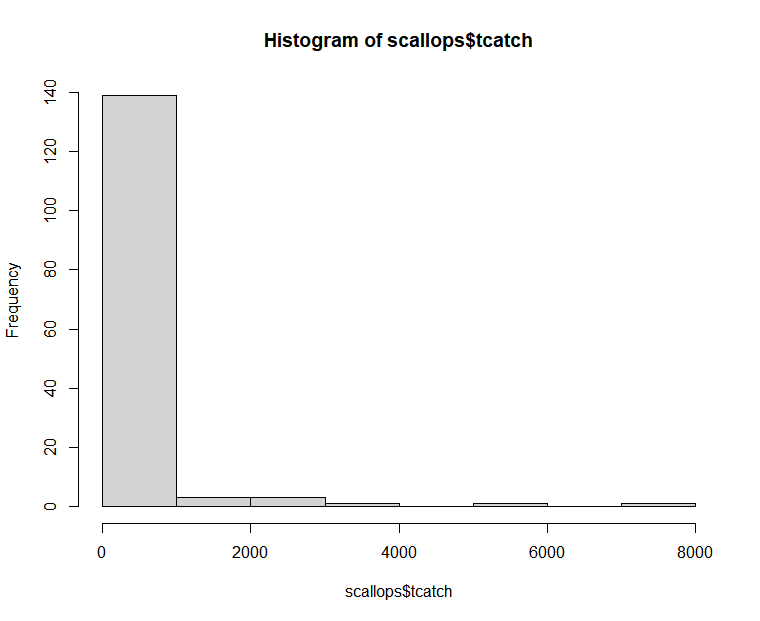
\includegraphics[width = .85\textwidth]{Rplot.png}
      \end{center}
    \end{figure}
    \begin{figure}[H]
      \begin{center}
      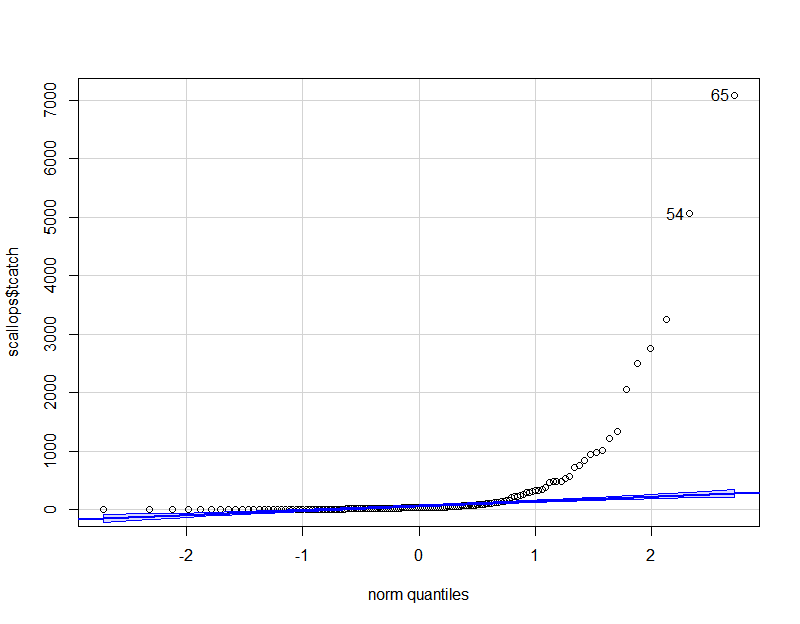
\includegraphics[width = .85\textwidth]{Rplot01.png}
      \end{center}
    \end{figure}
  \end{enumerate}
\end{exercise}
\vspace{1in}




\begin{exercise}{2} Log-transforming the scallops data.\\
  \begin{enumerate}


  \item Create a new column in the data set for a log-transformed total catch variable:\\
  \verb@    scallops$logcatch <- log( 1 + scallops$tcatch )@.\\
  Why did you need to add 1 before taking the logarithm?\\
  \solution Firstly we must add 1 to the total catch data before performing the transformation because
  the log(0) goes to minus infinity, and that goes for any base. Beyond that shifting the data by one shouldn't have 
  any appreciable difference in our EDA. After log transforming our data, looking at the summary report we can see that it 
  clearly reflects a more normal distribution with the mean and median being very close to each other and near the middle of the range.\\
  \textbf{Code:}
  \begin{center}
  \lstinputlisting[basicstyle = \footnotesize]{r2.txt}
  \end{center}
  \vspace{.15in}
  

  \item Is this natural log or log base 10? Would your plot differ in
  any meaningful way if you used the other base for the logarithm? Explain briefly.\\
  \solution Looking at the documentation we can see that when we use the log() function without the 
  base parameter the default is to use the natural log to transform the data. As discussed in exercise 7 from homework 
  2 that converting between the natural log and log base 10 transformation, involves multiplying 
  the whole data set by a constant. Therefore in terms of describing the histogram, the log base 10 transformation will 
  produce a more compact histogram, with a smaller range.   
  \vspace{.15in}

  
  
  \item Create a histogram and a normal probability plot 
  of logcatch; do the data appear more normally distributed
  than before?  Explain briefly.\\
  \solution Looking at the histogram we can see that we definitely have a more normal looking 
  distribution. This conclusion is corroborated by the fit of the qq plot. The large quantities of
  0 catch observations are something that we just have to deal with. When we go out and sample locations 
  we are not guaranteed to sample the signal(is the P(catching scallops = 0) or is our observation outside 
  of the support of the scallop catching probability distribution?). 

  \begin{figure}[H]
    \begin{center}
    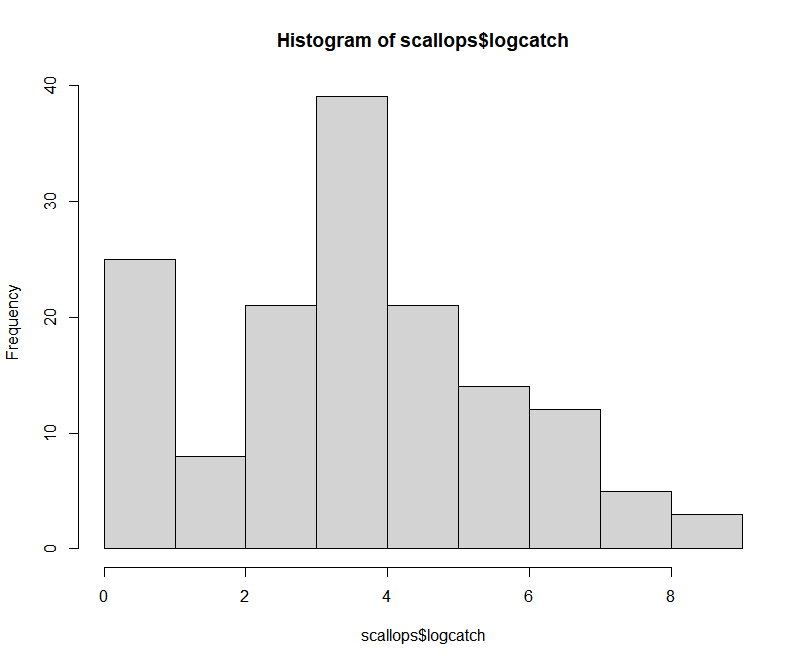
\includegraphics[width = .70\textwidth]{Rplot02.png}
    \end{center}
  \end{figure}
  \begin{figure}[H]
    \begin{center}
    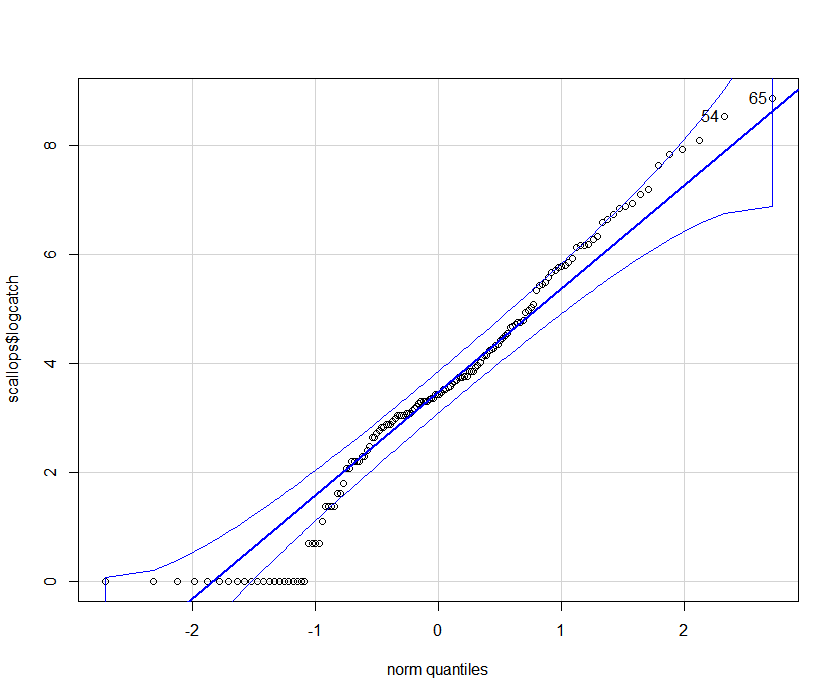
\includegraphics[width = .70\textwidth]{Rplot03.png}
    \end{center}
  \end{figure}

  \vspace{.15in}




  
  %\item Plot the locations of the data: 
  
  %\verb+   plot(scallops$long,scallops$lat,pch=16, xlab="lon",ylab="lat")+.
  
  \item Plot the data on top of a map, as follows.
    \begin{verbatim}
    install.packages("maps")
    library(maps)
    map("usa",xlim=c(-74,-71),ylim=c(38.0,41.5))
    points(scallops$long,scallops$lat, pch=4, col="gray")
    \end{verbatim}
    \solution Plotting the data, we get the following (I added log catch data to the col parameter, out of curiosity.)
    \begin{figure}[H]
      \begin{center}
        \caption{Scallop Locations}
      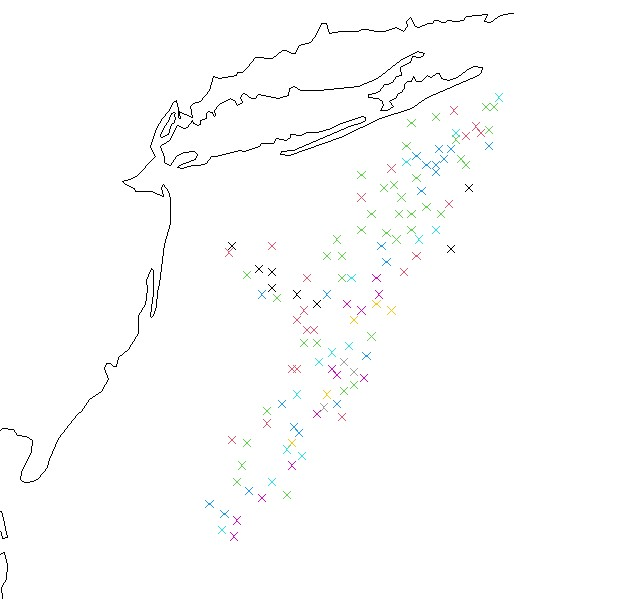
\includegraphics[width = .70\textwidth]{Rplot04.jpg}
      \end{center}
    \end{figure}
  \end{enumerate}
\end{exercise}
\vspace{1in}


\begin{exercise}{3}MLR with the scallops data.\\
  \begin{enumerate}
    \item Simple trend detection, using multiple linear regression (MLR).
      Fit the following MLR model, which assumes independent N(0,$\sigma^2$)
    errors.  Be sure to state the fitted
  model. (It's not enough to simply include the computer output, although you 
  should be doing that, too.)
  The model allows for linear and quadratic terms in latitude ($y$) or longitude ($x$).
    $$\mathbb{E}({\mbox{logcatch}}) = \beta_0 + \beta_1 x + \beta_2 y + \beta_3 x^2
    + \beta_4 y^2 + \beta_5 xy.$$
  
    The following R code fits this model and summarizes the parameter estimates and their
    standard errors, as well as $p$-values for the parameters:
    \begin{verbatim}
    scallops$clons <- scallops$long - mean(scallops$long)
    scallops$clats <- scallops$lat - mean(scallops$lat)
    myfit <- lm( logcatch ~ clons+clats + I(clons^2) +
                 I(clats^2) + I(clats*clons), data=scallops )
    summary(myfit)
    \end{verbatim}
    Does it appear that any trend terms might be appropriate?  Explain.  (I am looking
  for a formal hypothesis test or tests.)\\
  \solution Looking at the initial model summary, it appears as though the first order predictors have low significance. It could be 
  that the second order terms are capturing a larger portion of the variance, beyond that adding those terms makes the model harder to interpret
  especially the interaction term. Performing partial F-tests with the anova() function firstly on a first order model, and the second order model with no interaction, 
  we found that the second order predictors were significant. Testing the full second order model against the second order model with no interaction we found that 
  the interaction term was also significant.\\
  \textbf{Code:}
  \begin{center}
  \lstinputlisting[basicstyle = \footnotesize]{r3.txt}
  \end{center}
  \vspace{.15in}

  












  
  \item Why did I center the latitudes and longitudes? What would happen if I fitted
  the model without first centering the latitudes and longitudes? (Try it.)\\
  \solution
  \end{enumerate}
\end{exercise}
\vspace{1in}





\begin{exercise}{4} Choosing and fitting a (semi)variogram for the scallops data.\\
  \begin{enumerate}
  %\item Create a variogram cloud for these data (after detrending, if necessary).
  % Discuss briefly.
  \item  Plot the robust estimator for the variogram 
  (after detrending, if necessary). You may need to tweak this code:
  \begin{verbatim}
    geo.scallops <- as.geodata( 
      cbind(scallops$clons, scallops$clats, scallops$logcatch ))
    robust_est <- variog( geo.scallops,trend="2nd", estimator.type="modulus")
    plot(robust_est,pts.range=c(1,3),type='b')
  \end{verbatim}
  \solution From the previous problem we found that the second order model explained a significant amount 
  of the variance. Plotting the robust estimated semi variogram we get the following, 
  \begin{figure}[H]
    \begin{center}
      \caption{Robust estimator for the 2nd order semivariogram}
    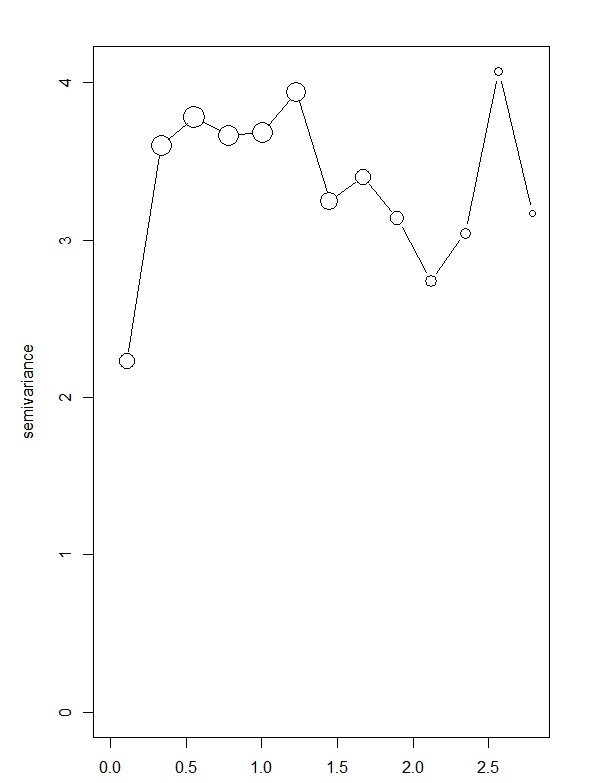
\includegraphics[width = .70\textwidth]{Rplot05.jpg}
    \end{center}
  \end{figure}
  









  
  
  \item Which theoretical semi-variogram appears to be most appropriate for these
  data? (Exponential, gaussian, spherical, or other?)
  Explain.  (It's entirely possible that there is no clear `winner'.)
  Does there appear to be a nugget?\\
  \solution Using the eyefit() function to get a sence of which semi-variogram model might be the most apporpriate we 
  get the following plots of the potential exponential, gaussian, and spherical semi-variograms. In every case we had a nugget of 
  around 1. From the shape of the model and the behavior of the parameters I feel as though the gaussian model is worth further exploration.\\  
  \textbf{Code:}
  \begin{center}
  \lstinputlisting[basicstyle = \footnotesize]{r4.txt}
  \end{center}
  \vspace{.15in}

  



  \begin{figure}[H]
    \begin{center}
      \caption{eyefit() Exponential Semi-variogram}
    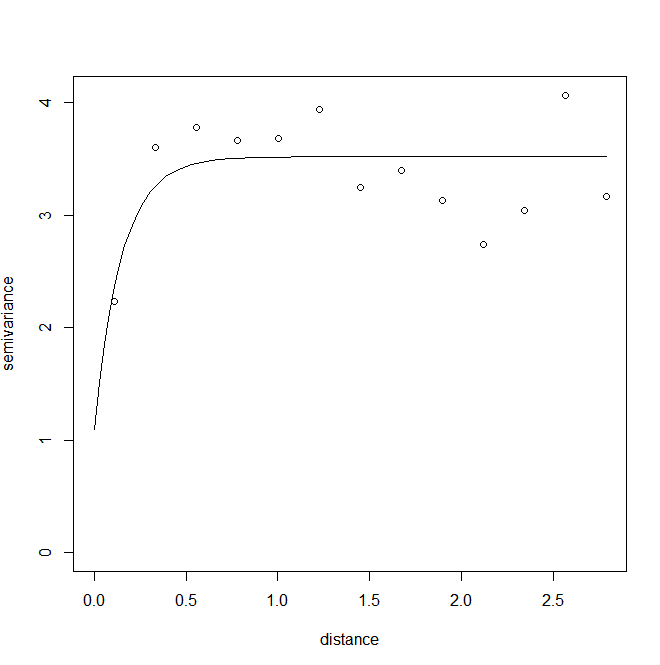
\includegraphics[width = .60\textwidth]{Exponential.png}
    \end{center}
  \end{figure}
  \begin{figure}[H]
    \begin{center}
      \caption{eyefit() Gaussian Semi-variogram}
    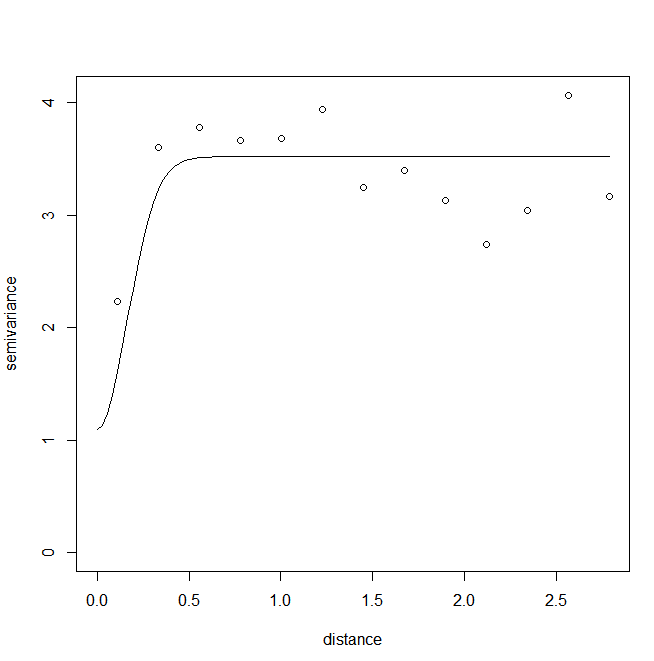
\includegraphics[width = .60\textwidth]{Gaussian.png}
    \end{center}
  \end{figure}
  \begin{figure}[H]
    \begin{center}
      \caption{eyefit() Spherical Semi-variogram}
    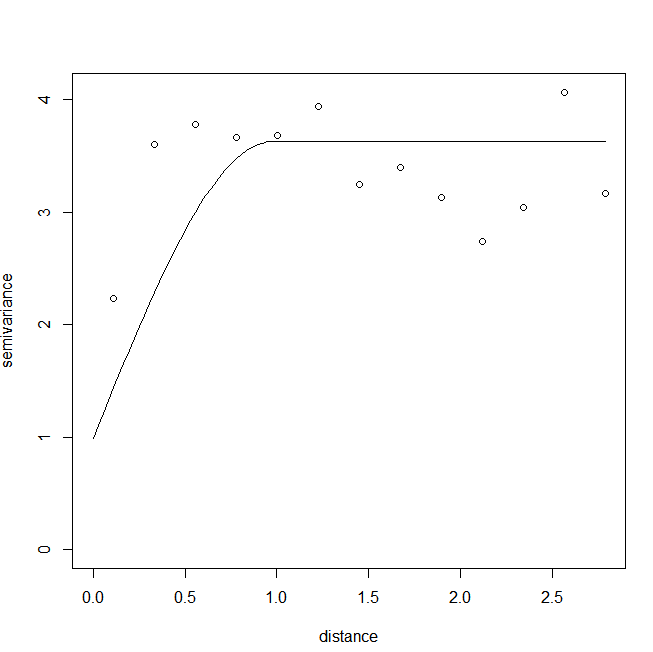
\includegraphics[width = .60\textwidth]{Spherical.png}
    \end{center}
  \end{figure}
  
  




  \item Fit your `winning' type of theoretical variogram 
  using the weighted least squares approach.
  State the resulting estimate for the theoretical variogram. You may need to tweak this code:
  \begin{verbatim}
    my_WLS_fit <- variofit( robust_est,
                            ini.cov.pars=c(2.0,.16),
                            cov.model="exponential",
                            fix.nugget=FALSE, nugget=2,
                            max.dist=1.9)
    my_WLS_fit$cov.pars; my_WLS_fit$nugget
  \end{verbatim}
  \solution Fitting the WLS estimator for a gaussian semi-variaogram we get the following semi-variogram,\\
  \textbf{Code:}
  \begin{center}
  \lstinputlisting[basicstyle = \footnotesize]{r5.txt}
  \end{center}
  \begin{figure}[H]
    \begin{center}
      \caption{WLS estimator for Gaussian semi-variogram}
    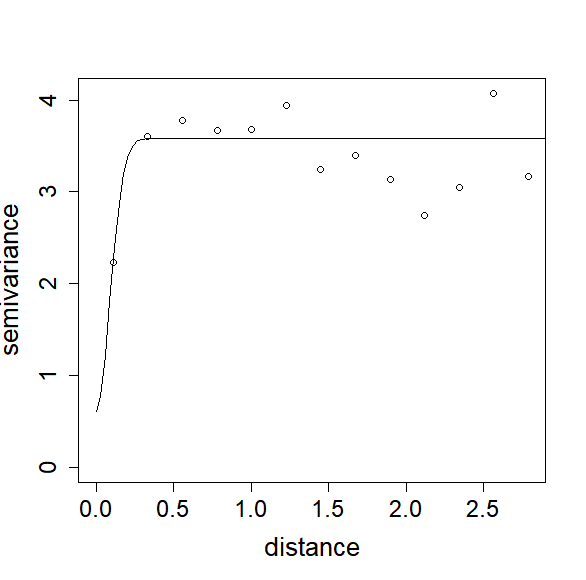
\includegraphics[width = .60\textwidth]{Rplot06.png}
    \end{center}
  \end{figure}
  



  



  

  \item Fit your `winning' theoretical variogram type
  using  maximum likelihohod (ML).  State the resulting estimates for the theoretical variogram.
  \begin{verbatim}
    ini_sigsq <- my_WLS_fit$cov.pars[1]
    ini_phi <- my_WLS_fit$cov.pars[2]
    ini_tausq <- my_WLS_fit$nugget
    my_ML_fit <- likfit( logCatch, trend="1st",
                         ini.cov.pars=c(ini_sigsq,ini_phi),
                         nugget=ini_tausq, lik.method="ML")
    c( my_ML_fit$sigmasq, my_ML_fit$phi, my_ML_fit$tausq)
  \end{verbatim}
  \solution Fitting the gaussian semi-variogram with the maximum likelihood algorithm we get the following, \\
  \textbf{Code:}
  \begin{center}
  \lstinputlisting[basicstyle = \footnotesize]{r6.txt}
  \end{center}
  \begin{figure}[H]
    \begin{center}
      \caption{ML estimator for Gaussian semi-variogram (WLS is dashed)}
    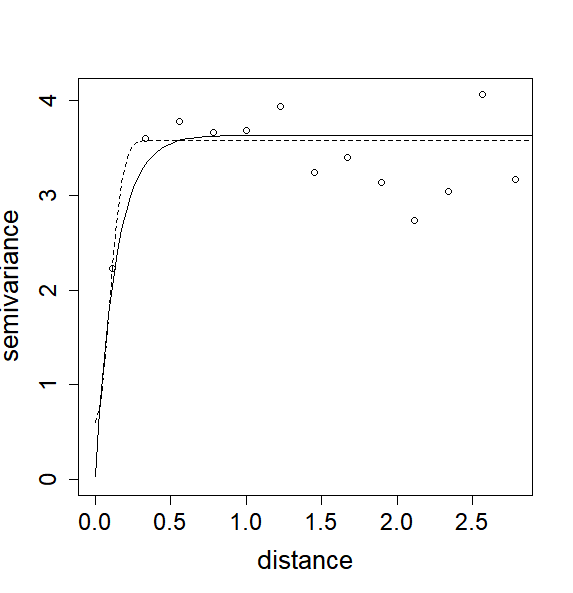
\includegraphics[width = .70\textwidth]{Rplot07.png}
    \end{center}
  \end{figure}

  













  
  
  \item Fit your winning theoretical variogram
  using REML.  State the resulting estimates for the theoretical variogram. Finaly graph all three semivariograms (WLS, ML, REML) on a single plot.
  \begin{verbatim}
    my_REML_fit <- likfit( logCatch, trend="2nd",
                           ini.cov.pars=c(ini_sigsq,ini_phi),
                           nugget=ini_tausq, lik.method="REML")
    c( my_REML_fit$sigmasq, my_REML_fit$phi, my_REML_fit$tausq)
  \end{verbatim}
  \solution  Fitting the gaussian semi-variogram with the residual maximum likelihood algorithm we get the following, \\
  \textbf{Code:}
  \begin{center}
  \lstinputlisting[basicstyle = \footnotesize]{r7.txt}
  \end{center}
  \begin{figure}[H]
    \begin{center}
      \caption{REML estimator for Gaussian semi-variogram (WLS is dashed)(ML is dotted)}
    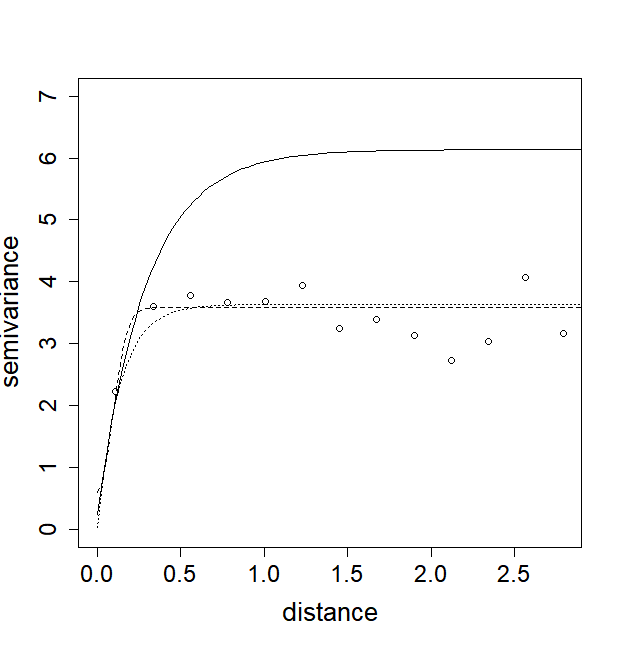
\includegraphics[width = .70\textwidth]{Rplot08.png}
    \end{center}
  \end{figure}
  

  \end{enumerate}
\end{exercise}
\vspace{1in}





\begin{exercise}{5} Simulating data, experimenting with estimating parameters for semivariograms.\\
  I have posted R code on Canvas for this assignment. The code carries out the following
  steps:
  \begin{itemize}
  \item It simulates a spatial
  data set using the geoR function, \verb+grf+. 
  \item It calculates and plots an empirical
  estimate of the semivariogram using the robust estimator. 
  \item It then carries out a
  randomization test to see whether a spatial model is necessary (which it should be,
  since we're using code to simulate spatial data!), and plots the results.
  \item  It overlays a curve that is the true semivariogram (the one that's used
  to simulate the original data)
  \item It overlays a curve that is an estimate of the semivariogram, using the WLS method.
  \end{itemize}
  
  Your instructions are to run the code 8 times, which results in 8 plots. The first four
  times you run the code, use $n=25$ observations; the second four times you run the
  code, use $n=100$ observations.
  
  \begin{enumerate}

  \item What type of semivariogram is the ``truth''? What are its parameters? Is there a nugget?\\
  \solution The ''truth'' semi-variogram is defined in the first block of code,\\
  \textbf{Code:}
  \begin{center}
  \lstinputlisting[basicstyle = \footnotesize]{r8.txt}
  \end{center}
  It describes the generation of random data with an exponential covariance function. This function 
  has parameters $\sigma^2 = 1.5$, $\phi = 10$, and $\tau^2 = 0$(The nugget parameter is set by default. This can be found in the grf() documentation.)
  \vspace{.15in}
  
  
  
  
  \item Summarize your results. Include a table for the parameter estimates for the $n=25$
  simulations and another table for the $n=100$ simulations.\\
  \solution Here are the results of our simulations, 
  \begin{figure}[H]
  \begin{center}
    \caption{Simulation results for $n = 25$}
    \begin{tabular}{|c||c|c|c| }
      \hline
      Trial & $\sigma^2$ & $\phi$ & $\tau^2$\\
      \hline 
      \hline
      1& 177.6862  & 3218.7565 &0\\
      2& 0.7664049 &  2.868407 &0\\ 
      3& 1.093023  & 6.151739 &0\\
      4& 27.77649  & 435.54335 &0\\
      \hline
     \end{tabular}
  \end{center}
\end{figure}

  \begin{figure}[H]
  \begin{center}
    \caption{Simulation results for $n = 100$}
    \begin{tabular}{|c||c|c|c| }
      \hline
      Trial & $\sigma^2$ & $\phi$ & $\tau^2$\\
      \hline 
      \hline
      1& 0.7267336 & 2.6374292  &0\\
      2& 1.541939  &  8.777938  &0\\ 
      3& 2.06919   &  12.03973 &0\\
      4& 1.104447  &  4.464463  &0\\
      \hline
     \end{tabular}
  \end{center}
\end{figure}
Since we know the true values of $\sigma^2 = 1.5$ and $\phi = 10$. It seems as though the first 
and fourth trials in the $n = 25$ simulation pulled a sample of observations which resulted in extremely large parameters in the 
WLS estimator. Generally it seems as though the WLS estimator for the $n = 100$ simulation performed better than the $n = 25$, this is 
as expected. When we look at the randomization tests, there is a lot less variation in the $n = 100$ simulation, it's easier to capture
 the signal of spatial correlation when we have more data. 

\begin{figure}[H]
  \begin{center}
    \caption{Resultant Plots from $n = 25$. Trials are plotted left to right, Trial 1 is top left \dots}
  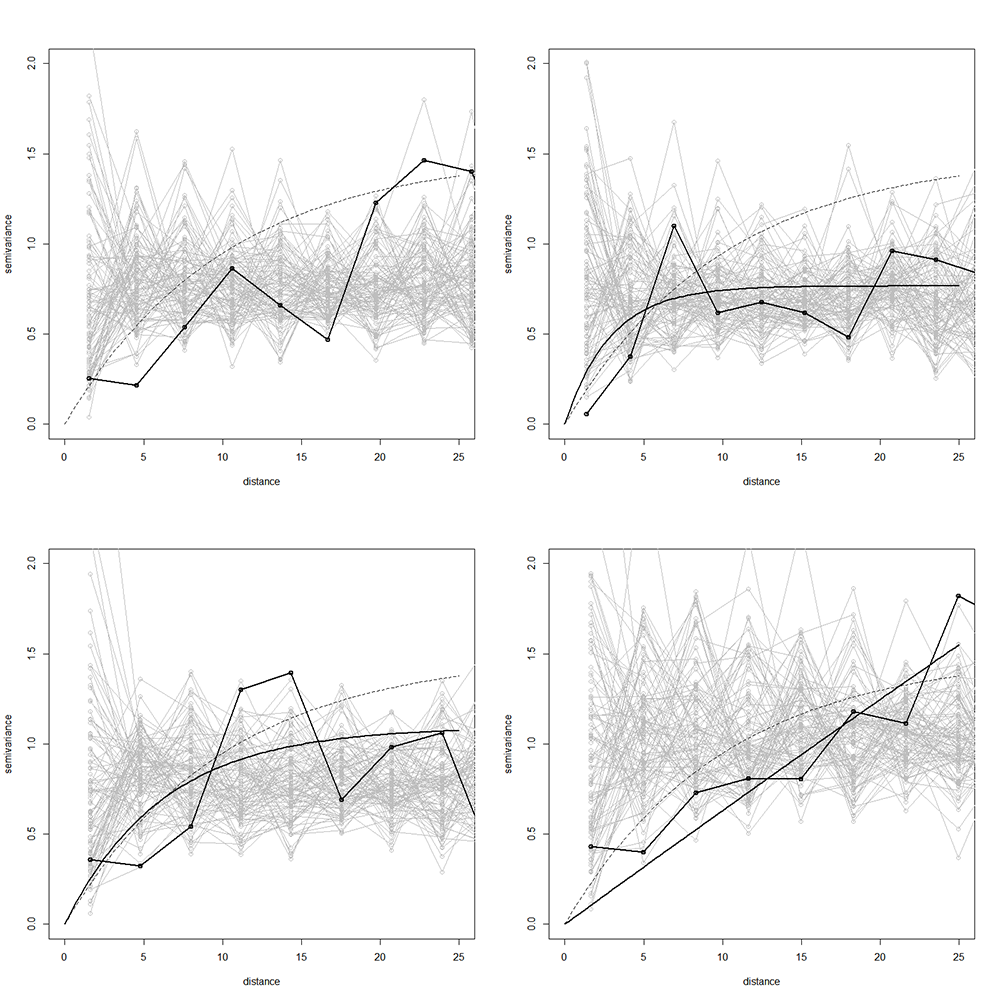
\includegraphics[width = \textwidth]{Group25.png}
  \end{center}
\end{figure}

\begin{figure}[H]
  \begin{center}
    \caption{Resultant Plots from $n = 100$. Trials are plotted left to right, Trial 1 is top left \dots}
  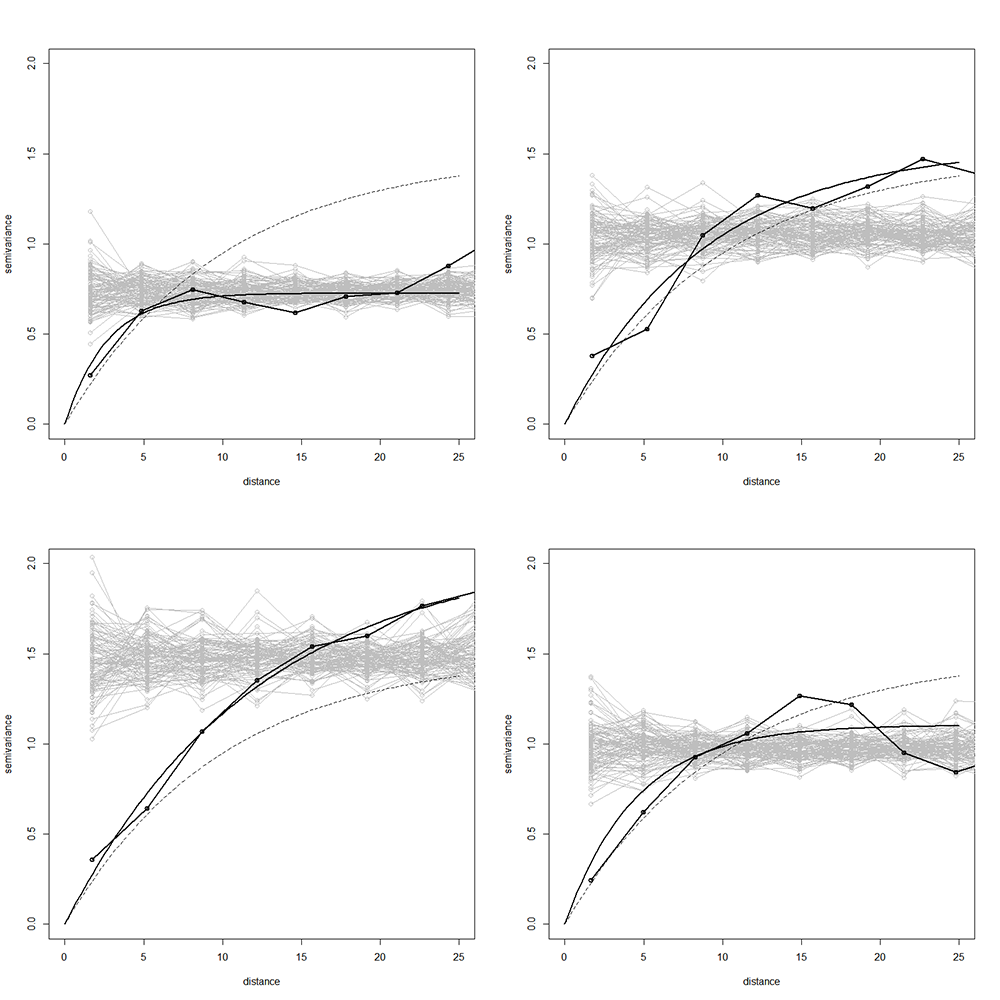
\includegraphics[width = \textwidth]{Group100.png}
  \end{center}
\end{figure}







  \item
  Do the empirical semivariograms appear to give a good match to the true semivariograms?
  Do the WLS estimated semiovariograms give a good match to the ``truth''? Do you get
  appreciably better results with the larger sample size? (One hopes that bigger sample
  sizes yield better estimates. Does this appear to be the case?)\\
  \solution Comparing the two simulations it seems that when we have a larger sample size the empirical semi-variogram will be closer 
  to the WLS estimated semi-variogram, not necessarily close to the true semi-variogram. Trials 1 and 3 of the $n = 100$ simulation did a poor 
  job of estimating the true semi-variogram even though we had more observations. I guess a possible conclusion is not that more observations is better, but 
  having observations that capture the spatial signal is better. It seems like trials 1 and 3 of the $n = 100$, ended up with a sample which failed to capture 
  the spatial signal as well as the other trials in the simulation. 
  
  
  
  
  
  \item
  Do the randomization tests appear to suggest that a spatial model is necessary in each case? 
  Explain briefly.\\
  \solution The randomization tests across both simulations suggest to me that a spatial model is necessary. Across all trials we see that 
  the empirical semi-variogram exhibits a trend that goes across the random semi-variograms. In the $n = 100$ simulation this trend is clearer, since we have more 
  observations there is less variance among the randomized semi-variograms.
  \end{enumerate}
  
\end{exercise}






\end{document}

